\documentclass[a4paper]{article}

\usepackage[nocomments]{latexml}
\usepackage{bookml/bookml}
\bmlImageEnvironment{tikzpicture}
\bmlImageEnvironment{tikzcd}
\let\ldsHTML\bmlRawHTML

\usepackage[pdfusetitle,colorlinks]{hyperref}
\usepackage[dvipsnames]{xcolor}

\usepackage{cmbright}

\usepackage{geometry}

\setlength{\parindent}{0pt}
\setlength{\parskip}{0.3em}

\usepackage{tabularx}
\renewcommand\tabularxcolumn[1]{m{#1}}% for vertical centering text in X column

\def\tikzname{Ti\emph{k}Z}
\iflatexml
\def\Xy{Xy}
\else
\usepackage[all]{xy}
\usepackage{tikz}
\usetikzlibrary{cd}
\fi

\usepackage{listings}
\lstset{basicstyle={\small\ttfamily},%
  keywordstyle={\color{blue}\bfseries},%
  keywordstyle=[2]{\color{MidnightBlue}\bfseries},%
  stringstyle={\color{red}},%
  commentstyle={\color{OliveGreen}},%
}

\lstdefinestyle{latexml}{language=[LaTeX]TeX,%
  texcsstyle=*{\color{blue}\bfseries},%
  texcsstyle=*[2]{\color{MidnightBlue}\bfseries},%
  moretexcs=[2]{LaTeXML,iflatexml,lxAddClass,lxWithClass,lxBeginTableHead,lxEndTableHead,lxFcn,lxID,lxPunct,lxContextTOC,lxNavbar,lxHeader,lxFooter,ldsHTML,bmlRawHTML,bmlImageEnvironment,bmlDescription,}%
  moretexcs={chapter,text,}%
  }

\def\ltxinline{\lstinline[style=latexml,frame=none]}

\usepackage{amsthm}
\theoremstyle{definition}
\newtheorem{exa}{Example}[subsection]

\title{LaTeXML + BookML guide}
\author{Vincenzo Mantova}

\date{3 September 2021}

\begin{document}

\maketitle

\begin{abstract}
  This is a short guide to \LaTeXML{} and the \href{https://vlmantova.github.io/bookml/}{BookML} add-on in order to produce (hopefully!) WCAG 2.1 AA compliant documents out of your \LaTeX{} files, with minimal changes to your \verb|.tex| code. The add-on gives you access to a bookdown-style output (optional), alternative text for images, direct output of \HTML{} (for instance to embed videos). This very document is written in \LaTeX{} and converted to \HTML{} in this way.

  The hard work is done by \LaTeXML{}. If you want to see \LaTeXML{} in action, you can visit \href{https://www.arxiv-vanity.com/}{arXiv Vanity} and paste the link to one of your own preprints, or you can use the online \href{https://latexml.mathweb.org/editor}{demo \LaTeX{} editor} to type \LaTeX{} and check the \HTML{} output right in the browser (the page has several advanced examples, including \tikzname{} pictures).
\end{abstract}

\begin{center}
  Formats: \href{https://minerva.leeds.ac.uk/bbcswebdav/courses/201920_MAPS_MM8863/latexmlleeds/}{HTML} (bookdown style), \href{https://minerva.leeds.ac.uk/bbcswebdav/courses/201920_MAPS_MM8863/latexmlleeds/index.plain.html}{HTML} (plain style), \href{https://minerva.leeds.ac.uk/bbcswebdav/courses/201920_MAPS_MM8863/latexmlleeds/LaTeXML-Leeds.epub}{EPUB}, \href{https://minerva.leeds.ac.uk/bbcswebdav/courses/201920_MAPS_MM8863/latexmlleeds/LaTeXML-Leeds.pdf}{PDF}.
\end{center}

\subsection*{Recent changes}
\subsubsection*{2021/09/03}
The \texttt{latexmlleeds} additions have now become a tiny addition to \href{https://vlmantova.github.io/bookml/}{BookML}, which is very similar, but a lot better, faster, and easier to use. If you already use \texttt{latexmlleeds}, you can add a small compatibility layer to keep working (almost exactly) as before: see \autoref{sub:comp-latexmlleeds}.

\tableofcontents

\section{Installation}

\subsection{\texorpdfstring{\LaTeXML{}}{LaTeXML}}
Let me stress first: you must use \LaTeXML{} version 0.8.5 or newer. Check with
\begin{lstlisting}
  latexml --version
\end{lstlisting}
and upgrade if you see 0.8.4 or less. Version 0.8.6 should come out in September and I strongly recommend you keep an eye on it, because it contains many improvements (and it is a bit faster).

\subsubsection*{Windows}
\begin{itemize}
  \item For University machines (including the Windows Virtual Desktop): use \href{https://it.leeds.ac.uk/it?id=kb_article&sysparm_article=KB0014827}{AppsAnywhere} (for now, only when working online) or contact IT.
  \item Install \href{https://strawberryperl.com/}{StrawberryPerl} (\texttt{64bit}) (available on AppsAnywhere).
  \item In StrawberryPerl, run
    \begin{lstlisting}
cpanm --notest --verbose LaTeXML
    \end{lstlisting}
  \item Optional (for proper image handling): install \href{https://imagemagick.org/script/download.php}{ImageMagick} \texttt{x64-dll}, and if you have PDF or EPS pictures, add \href{https://www.ghostscript.com/download/gsdnld.html}{Ghostscript} 64 bit (both available on AppsAnywhere). Then run
    \begin{lstlisting}
cpanm --verbose Image::Magick
    \end{lstlisting}
  \item Optional (for BookML additional image functionality): ensure your \LaTeX{} installation comes with \texttt{latexmk}, \texttt{dvisvgm}, \texttt{preview.sty}.
\end{itemize}

\subsubsection*{macOS}
MacPorts is the best option (\href{https://dlmf.nist.gov/LaTeXML/get.html}{instructions}). \href{https://nixos.wiki/wiki/Nixpkgs}{Nixpkgs} is very solid, if you know how to use it (the package is \texttt{perlPackages.LaTeXML}).

You can also use \href{https://brew.sh/}{Homebrew} but you will miss some image functionality.

Finally, you might be able to get a fully functional LaTeXML via:
\begin{lstlisting}
cpan LaTeXML
cpan Image::Magick 
\end{lstlisting}

\subsubsection*{Linux}
Many distributions include the package \texttt{latexml}, \textbf{but it is often outdated}. Check if you can find \texttt{.deb} or \texttt{.rpm} files for versions 0.8.5, or soon 0.8.6, from more up-to-date distributions (e.g.\ Debian Unstable, Fedora).

\subsection{BookML}
Unpack BookML next to your \texttt{.tex} files as instructed in the \href{https://vlmantova.github.io/bookml/}{BookML manual}. Then add
\begin{lstlisting}[style=latexml]
\usepackage{bookml/bookml}
\end{lstlisting}
anywhere in your preamble.

\subsection{Compatibility with \texttt{latexmlleeds}}
\label{sub:comp-latexmlleeds}
If you have been using \texttt{latexmlleeds}, replace \ltxinline|\usepackage{latexmlleeds}| in your preamble with the following:
\begin{lstlisting}[style=latexml]
\usepackage[style=plain]{bookml/boomkl}
\bmlImageEnvironment{tikzpicture} % if using tikzextern
\bmlImageEnvironment{tikzcd}      % if using tikzcd
\let\ldsHTML\bmlRawHTML           % if using \ldsHTML
\end{lstlisting}
Moreover, put the \texttt{bmluser} folder from \href{bmluser-latexmlleeds.zip}{this file} next to your \texttt{.tex} files.

\ltxinline|tikzextern| users will like to know that BookML has a massively faster and fully automated way of generating images. No need for \ltxinline|-shell-escape|, \ltxinline|pdf2svg|, or other additional steps.

If the \tikzname{} pictures have the wrong size, try adding the option \lstinline|imagescale=X.XX| (read the BookML manual for the details).

I suggest you try removing \ltxinline{[style=plain]} and see if the bookdown style is suitable for your material.

\section{How to use \texorpdfstring{\LaTeXML{}}{LaTeXML} and BookML}
A piece of advice: if you are not familiar with \LaTeXML{}, start with a small document first. For instance, put \ltxinline|\end{document}| early, like after a single section. Once you get things working, you can go with the entire document.

\subsection{Getting the \HTML{} out}
\begin{enumerate}
  \item Install everything as above.
  \item Do you have many \tikzname{} pictures (say more than 10)? You may want to apply the \tikzname{} instructions in \autoref{sub:tweaks} right away and save some time.
  \item Run
  \begin{lstlisting}[language=bash]
latexml --destination=myfile.xml myfile.tex
  \end{lstlisting}
  If it fails because of \texttt{Fatal}'s, bisect with \ltxinline|\end{document}| to find the source of the problem. Once identified the problem, use \ltxinline|\iflatexml| to run alternative code under \verb|latexml|:
  \begin{lstlisting}[style=latexml]
\iflatexml
  % code only executed by latexml
\else
  % code only executed by other engines
\fi
  \end{lstlisting}
  Do not try to fix \texttt{Error}'s at this stage (some may be irrelevant anyway), unless they make \LaTeXML{} die.
  \item Conclude with
  \begin{lstlisting}[language=bash]
# to create the final HTML...
latexmlpost --navigationtoc=context \
  --destination=mynotes/myfile.html myfile.xml
# ...and zip it for upload on Minerva
zip -r mynotes.zip mynotes
  \end{lstlisting}
  Do create a subfolder (the \verb|mynotes| in \verb|mynotes/myfile.html| above) since there are additional files that need to travel with the main \verb|myfile.html|.
\end{enumerate}

\subsection{Adjust and fix}
\label{sub:tweaks}

After you have made \LaTeXML{} happy, you likely need to adjust the end result, or to fix some errors.

\begin{description}
  \item[Split large documents.] Add \verb|--splitat=| to \verb|latexmlpost| to split the output in various ways (part, chapter, section\dots{}). You \textbf{must} split long documents, or MathJax will take ages to render your formulas.
  \item[Disable the bookdown style.] If you do not like the bookdown style and prefer a more plain page, like the old \texttt{latexmlleeds}, use
  \begin{lstlisting}[style=latexml]
\usepackage[style=plain]{bookml/bookml}
  \end{lstlisting}
  or pass \lstinline|--preload=[style=plain]bookml/bookml| when calling \texttt{latexml}. You may wish to remove \lstinline| --navigationtoc=context| (see below about sidebars).
  \item[Navigation sidebar.] This is already included in the bookdown style. If you disable it, though, but still want the sidbar, add \verb|--css=LaTeXML-navbar-left.css| to \verb|latexmlpost|.
  \item[Customise CSS (fonts, color).] Create the \texttt{bmluser} and add any CSS file to it.
  \item[Alternative text for images.] Add \ltxinline|\bmlDescription{text}| right after the image (do not leave an empty line between the image and the text). This will populate the \texttt{alt} attribute (or equivalent) and will be read by screen readers in place of the image.

    Please keep in mind that sighted users may also benefit from the alternative text. If that is the case, consider using \ltxinline|\begin{figure}| and \ltxinline|\caption{}|, and possibly add a reference in the caption to more explanations (e.g.\ the definition, a proof, etc.).
  \item[Many or complex \tikzname{} pictures] BookML has a facility to generate the images via \LaTeX{}, and bypassing \LaTeXML{}'s slow support for \tikzname{} altogether.

  Ensure that all of the \tikzname{} code is either in the preamble or between \ltxinline|\begin{tikzpicture}| and \ltxinline|\end{tikzpicture}|, then add the following to the preamble, after the bookml package:
\begin{lstlisting}[style=latexml]
\bmlImageEnvironment{tikzpicture}
\bmlImageEnvironment{tikzcd} % if using tikzcd
\iflatexml
\else
\usepackage{tikz}
% ... ALL other TikZ-related set up
\fi
\end{lstlisting}
    See \autoref{fig:tikz-example}, \autoref{fig:tikzcd-example}.
  \item[\Xy-matrices, \texttt{animate}.] Most packages producing pictures are not supported by \LaTeXML{}, but you can get around it exactly like with \tikzname{}. If pictures are their own environment, use \ltxinline|\bmlImageEnvironment| as for \tikzname{}: see \autoref{fig:xymatrix-example}. If not, you can wrap images between \ltxinline|\begin{bmlimage}| and \ltxinline|\end{bmlimage}|. You can read more details and see examples in \href{https://vlmantova.github.io/bookml}{BookML manual}.
  \item[Embed videos.] You can use \ltxinline|\bmlRawHTML{html}| to write arbitrary \HTML{}, in particular output the embedding code for Stream, Mediasite, YouTube, or any other platform. See \autoref{fig:embed-stream} below for some reusable code that will also make the video adapt to the size of the page.
  \item[Unsupported packages.] \LaTeXML{} supports only so many packages (\href{https://dlmf.nist.gov/LaTeXML/manual/included.bindings/}{full list}). If your package is not supported, or is not supported well, see \autoref{sub:unsupported-packages}.
  \item[Broken links in formulas.] You \textbf{cannot} use anything other than text in \ltxinline|\mbox{},\text{}| when inside an equation. This is a limitation of MathJax. Long-term, BookML will automatically strip non-text content but for now you have to do it yourself (for instance, remove references or replace \ltxinline|\ref| with \ltxinline|\ref*| where applicable).
  \item[Table headers.] You may need to explicitly mark some table rows as headers. This can be done with some appropriate commands provided by \LaTeXML{}. See \autoref{fig:table} for an example.
  \item[Embed \TeX{} code as annotation.] I recommend including the \TeX{} code in your mathematical formulas. It can be accessed by right-clicking on the formulas. Use \ltxinline|--pmml --mathtex| when calling \ltxinline|latexmlpost| to do that.
  \item[Other options.] Visit the \href{https://dlmf.nist.gov/LaTeXML/docs.html}{\LaTeXML{} documentation} or run \verb|latexml --help|, \verb|latexmlpost --help|, \verb|latexmlc --help|.
\end{description}

\subsection{Unsupported packages}
\label{sub:unsupported-packages}
There are a few ways to deal with an unsupported package, as long as the package is doing something simple, like introducing convenience macros or producing images.
\begin{itemize}
  \item If the package is producing images, see the instructions above about \ltxinline|\bmlImageEnvironment| and \ltxinline|\begin{bmlimage}|.
  \item Replace the package with a suitable equivalent supported by \LaTeXML{}.
  \item Use \ltxinline|\iflatexml| and \ltxinline|\newcommand| in the preamble to define the macros you need so that they do something equivalent. Good if the macros are only for the PDF (e.g.\ it refers to page numbers, it applies a certain style, etc.), or if similar functionality is provided by a \LaTeXML{}-supported package but you do not want to change package altogether.
  \item Copy the missing definition from the package itself and add it to your preamble (usually within \ltxinline|\makeatletter| and \ltxinline|\makeatother|). It might work with packages partially supported by \LaTeXML{} and only missing a few bits.
  \item If \verb|package| is not supported by \LaTeXML{}, paste the following code in the file \verb|package.sty.ltxml| and put it in the same folder as the \verb|.tex| file (replace \verb|sty| with \verb|cls| if dealing with a class):
  \begin{lstlisting}[language=Perl]
use LaTeXML::Package;
InputDefinitions('package', type => 'sty', noltxml => 1);
1;
  \end{lstlisting}
  This tells \LaTeXML{} to read \texttt{package.sty}.
\end{itemize}

If none of the easy solutions work, you may need a new `binding' for the package, and that is not an easy task.

\begin{figure}
  \begin{center}
    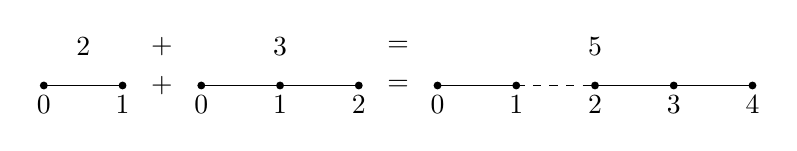
\begin{tikzpicture}
      \draw (0.5,0.5) node {$2$};
      \draw (1.5,0.5) node {$+$};
      \draw (3,0.5) node {$3$};
      \draw (4.5,0.5) node {$=$};
      \draw (7,0.5) node {$5$};
      \draw (0,0) node [below] {$0$} -- (1,0) node [below] {$1$};
      \draw (1.5,0) node {$+$};
      \draw (2,0) node [below] {$0$} -- (3,0) node [below] {$1$} -- (4,0) node [below] {$2$};
      \draw (4.5,0) node {$=$};
      \draw (5,0) node [below] {$0$} -- (6,0) node [below] {$1$};
      \draw [dashed] (6,0) -- (7,0);
      \draw (7,0) node [below] {$2$} -- (8,0) node [below] {$3$} -- (9,0) node [below] {$4$};
      \foreach \x in {0,1,2,3,4,5,6,7,8,9} {
        \fill (\x,0) circle (0.05);
      }
    \end{tikzpicture}
  \end{center}
  \bmlDescription{To compute 2+3, add a copy of the well ordered set 3 after the well ordered set 2, and note that the result is isomorphic to the well ordered set 5.}
  \caption{Ordinal sum of $2$ and $3$ (note that the image has an alternative text!).}
  \label{fig:tikz-example}
\end{figure}

\begin{figure}
  \begin{center}
    \begin{tikzcd}
      A \arrow[rd] \arrow[r, "\phi"] & B \\
                                      & C
    \end{tikzcd}
    \bmlDescription{A, B, C drawn in a triangle with C under B, an arrow labelled phi from A to B and an arrow from A to C}
  \end{center}
  \caption{Example of tikzcd diagram.}
  \label{fig:tikzcd-example}
\end{figure}

\begin{figure}
  \begin{lstlisting}[style=latexml]
\begin{bmlimage}
  \[ \xymatrix{
        A \ar[rd] \ar^\phi[r] & B \\
                              & C } \]
\end{bmlimage}
\bmlDescription{A, B, C drawn in a triangle with C under B,
  an arrow labelled phi from A to B and an arrow from A to C}
  \end{lstlisting}
  \begin{center}
    \begin{bmlimage}
      \[ \xymatrix{
            A \ar[rd] \ar^\phi[r] & B \\
                                  & C } \]
    \end{bmlimage}
    \bmlDescription{A, B, C drawn in a triangle with C under B, an arrow labelled phi from A to B and an arrow from A to C}
  \end{center}
  \caption{Example of \Xy-matrix diagram.}
  \label{fig:xymatrix-example}
\end{figure}

\begin{figure}
  \begin{lstlisting}[style=latexml]
% preamble
\newcommand{\includestream}[2]{
  \bmlRawHTML{<div style="max-width: 1920px; width: 100\%">
    <div style="position: relative; padding-bottom: 56.25\%; height: 0; overflow: hidden;">
      <iframe
        src="https://web.microsoftstream.com/embed/video/#1?autoplay=false\&amp;showinfo=true"
        title="#2" style="border:none; position: absolute; top: 0; left: 0;
          right: 0; bottom: 0; height: 100\%; max-width: 100\%;"
        allow="picture-in-picture" allowfullscreen="" width="1920" height="1080">
      </iframe>
    </div></div>}
    Watch \href{https://web.microsoftstream.com/video/#1}{#2}
  }
% document
\includestream{ba6b8866-df29-4dea-a47e-13decc5cd409}{Mock recording for Models and Sets}
  \end{lstlisting}
  \begin{quote}
    \newcommand{\includestream}[2]{
      \bmlRawHTML{<div style="max-width: 1920px; width: 100\%">
        <div style="position: relative; padding-bottom: 56.25\%; height: 0; overflow: hidden;">
          <iframe
            src="https://web.microsoftstream.com/embed/video/#1?autoplay=false\&amp;showinfo=true"
            title="#2" style="border:none; position: absolute; top: 0; left: 0;
              right: 0; bottom: 0; height: 100\%; max-width: 100\%;"
            allow="picture-in-picture" allowfullscreen="" width="1920" height="1080">
          </iframe>
        </div></div>}
        Watch \href{https://web.microsoftstream.com/video/#1}{#2}
      }
      % document
      \includestream{ba6b8866-df29-4dea-a47e-13decc5cd409}{Mock recording for Models and Sets}
  \end{quote}
  \label{fig:embed-stream}
  \caption{How to embed a video. Note that the \LaTeX{} special characters are preceeded by a backslash or the output may be invalid.}
\end{figure}

\begin{figure}
  \begin{lstlisting}[style=latexml]
% before \usepackage{bookml/bookml}
\usepackage[nocomments]{latexml}
% document
\begin{tabularx}{\textwidth}{c|X||c}
  \lxBeginTableHead{} Header 1 & Header 2 & Header 3 \\
  \hline \lxEndTableHead{}
  Content & Content & Content \\
  More content & content & content \\
  \hline
\end{tabularx}
\caption{A table}
  \end{lstlisting}
  \begin{tabularx}{\textwidth}{c|X||c}
    \lxBeginTableHead{} Header 1 & Header 2 & Header 3 \\
    \hline \lxEndTableHead{}
    Content & Content & Content \\
    More content & content & content \\
    \hline
  \end{tabularx}
  \caption{Mark a table row as header. If your \LaTeX{} installation does not have \texttt{latexml.sty}, you can download it from the \href{https://github.com/brucemiller/LaTeXML/blob/master/lib/LaTeXML/texmf/latexml.sty}{LaTeXML source}. Read the content of \texttt{latexml.sty} for more table-related commands.}
  \label{fig:table}
\end{figure}

\subsection{The \texttt{latexml} package (advanced)}
\begin{lstlisting}[style=latexml,caption={Import \texttt{latexml} in the preamble}]
  \usepackage[nocomments]{latexml}
\end{lstlisting}

The package \verb|latexml| takes some options that will be passed to the \LaTeXML{} engine, such as \ltxinline|nocomment| (that strips the \ltxinline|%| comments away) or \ltxinline|mathparsespeculate|. Moreover, it offers a variety of commands which may be useful. Just open \href{https://github.com/brucemiller/LaTeXML/blob/master/lib/LaTeXML/texmf/latexml.sty}{\texttt{latexml.sty}} (it is very short) to see all the commands, a bit of documentation in the comments, and the occasional example. The \href{https://github.com/brucemiller/LaTeXML/tree/master/doc/manual}{source} of the \LaTeXML{} documentation is contains many examples too.
\begin{itemize}
  \item \ltxinline|\lxAddClass{class}| and \ltxinline|\lxWithClass{class}{content}| to add \CSS{} classes to the output;
  \item \ltxinline|\lxBeginTableHead|, \ltxinline|\lxEndTableHead| and variations to mark table headers and footers (read the \verb|latexml.sty| source for how to use them);
  \item \ltxinline|\lxFcn{code}|, \ltxinline|\lxID{code}|, \ltxinline|\lxPunct{code}| to help \LaTeXML{} understand the meaning of mathematical symbols (\LaTeXML{} recognises the meaning on its own, but every once in a while, there will be a symbol that is just too ambiguous: is $f(a+b)$ the function $f$ applied to $a+b$, or the number $f$ multiplied by $a+b$? keep an eye on the warnings during compilation);
  \item \ltxinline|\lxContextTOC|, \ltxinline|\lxNavbar{arg}|, \ltxinline|\lxHeader{arg}|, \ltxinline|\lxFooter{arg}| to customise the HTML pages (I have yet to figure out how they work);
  \item and a few other commands.
\end{itemize}

\appendix

\section{Other documentation}
\begin{itemize}
  \item \href{https://dlmf.nist.gov/LaTeXML/docs.html}{\LaTeXML{} documentation}
  \item List of packages \href{https://dlmf.nist.gov/LaTeXML/manual/included.bindings/}{supported by \LaTeXML{}} (note that some implementations are not complete)
  \item \href{http://docs.mathjax.org/en/v2.7-latest/}{MathJax v2.7} documentation
  \item List of \LaTeX{} commands \href{http://docs.mathjax.org/en/v2.7-latest/tex.html#supported-latex-commands}{supported by MathJax v2.7}
  \item \href{http://docs.mathjax.org/en/v3.2-latest/}{MathJax v3.2} documentation
  \item List of \LaTeX{} commands \href{http://docs.mathjax.org/en/v3.2-latest/input/tex/macros/index.html}{supported by MathJax v3.2}
\end{itemize}

\section{Past changes}

\subsubsection*{2021/01/13}
\begin{itemize}
  \item \verb|docs|: you \textbf{must use} \ltxinline|\usepackage[nocomments]{latexml}| (i.e., add the option \verb|nocomments|) if you want to use the \verb|tikzextern| option of \verb|latexmlleeds|. \verb|tikzextern| is very likely to fail if you do not. The guide has been updated accordingly.
  \item \verb|docs|: changes moved to the end of the document.
\end{itemize}
\subsubsection*{2021/01/11}
\begin{itemize}
  \item \verb|latexmlleeds|: improve the mobile experience in presence of content (such as images) larger than the device screen. Previously, the browser would shrink the entire page to make the images fit, now it will show the page at 100\% zoom and allow horizontal scrolling for the overflowing content.
  \item \verb|latexmlleeds|: invisible TikZ improvements.
  \item \verb|docs|: since \LaTeXML{} v0.8.5, \textbf{use} \verb|--pmml| before \verb|--mathtex| when invoking \verb|latexmlpost|.
  \item \verb|docs|: support for \LaTeXML{} v0.8.4 will eventually be dropped. Please upgrade to v0.8.5 as soon as you can.
\end{itemize}
\subsubsection*{2020/09/24}
\begin{itemize}
  \item \verb|css|: fix a problem with nested ordered lists not making any sense (sorry!).
  \item \verb|docs|: clarify that \verb|tikzpicture| and \verb|tikzcd| are not supported in mathematical mode.
  \item \verb|docs|: explain that \verb|xymatrix| is not supported.
\end{itemize}
\subsubsection*{2020/09/17}
\begin{itemize}
  \item \verb|latexmlleeds|: scale TikZ images properly regardless of the availability of ImageMagick. The behaviour can be tuned with the option \verb|tikzscale=factor|.
  \item \verb|latexmlleeds|: implement an additional TikZ workaround for \verb|tikz-cd| that can be enabled by passing the option \verb|tikzcd|.
  \item \verb|latexmlleeds|: the TikZ workaround is more robust and it requires even fewer changes (you do not need to import \verb|graphicx| or \verb|external| explicitly any more).
\end{itemize}
\subsubsection*{2020/09/07+\texorpdfstring{$\varepsilon$}{ɛ}}
\begin{itemize}
  \item \verb|latexmlleeds|: make TikZ workaround implementation compatible with the previous approach, so that the old code and the new can coexist without changes.
\end{itemize}
\subsubsection*{2020/09/07}
\begin{itemize}
  \item \verb|latexmlleeds|: rename \ltxinline|\lxHTML| to \ltxinline|\ldsHTML| to distinguish \verb|latexml| commands from the Leeds additions; \ltxinline|\lxHTML| is retained for backward compatibility.
  \item \verb|latexmlleeds|: the additional \CSS{}, the custom \XSLT{}, and MathJax are now loaded automatically, simplifying considerably the calls to \verb|latexml| and \verb|latexmlpost| (in particular: \verb|latexmlleeds-html5.xsl| has been renamed \verb|LaTeXML-html5.xsl|, so delete the old file after downloading the new one). \textbf{Warning:} you must stop using the \verb|--stylesheet|, \verb|--css| and \verb|--javascript| options from the pre-2020/09/07 instructions, unless it is for your own customizations.
  \item \verb|latexmlleeds|: fully integrate the TikZ workaround with the package options \verb|tikzextern| and \verb|tikz2svg|.
  \item \verb|docs|: improve syntax colouring of \LaTeX{} snippets (accidentally revealing a bug in the \LaTeXML{} binding for the package \verb|listings|).
  \item \verb|docs|: explain how to deal with unsupported packages in a more sophisticated way, short of writing your our \LaTeXML{} binding.
  \item \verb|docs|: improve the video embedding example using the code provided by Microsoft when asking for a `responsive' embedded video.
\end{itemize}
\subsubsection*{2020/08/26}
\begin{itemize}
  \item Initial release.
\end{itemize}

\end{document}
